% !TEX root = ../MemPod.tex
\section{Results}
\label{sec:Results}

\subsection{Evaluation Framework}
\label{sub:Evaluation}

The goal of our evaluation framework is to quantitatively and qualitatively assess MemPod's capabilities and compare it against state-of-the-art proposed mechanisms. Throughout our evaluation section, we study MemPod's performance running with an eight-core CPU. We extend Ramulator \cite{kim-ramulator} to support flat address space hybrid memories. We model the MemPod architecture,
as well as HMA, THM and CAMEO in our simulation framework. Ramulator enables 
cycle-level memory simulation and includes a simple CPU front-end capable of approximating resource-induced stalls. We chose to evaluate MemPod under a realistic memory configuration consisting of 1GB 3D-stacked HBM \cite{JEDEC-HBM-REVISED} and 8GB of off-chip DDR4-1600. Table \ref{tab:specs} Provides a more detailed description of the simulated system's configuration.

\begin{table}[t]
  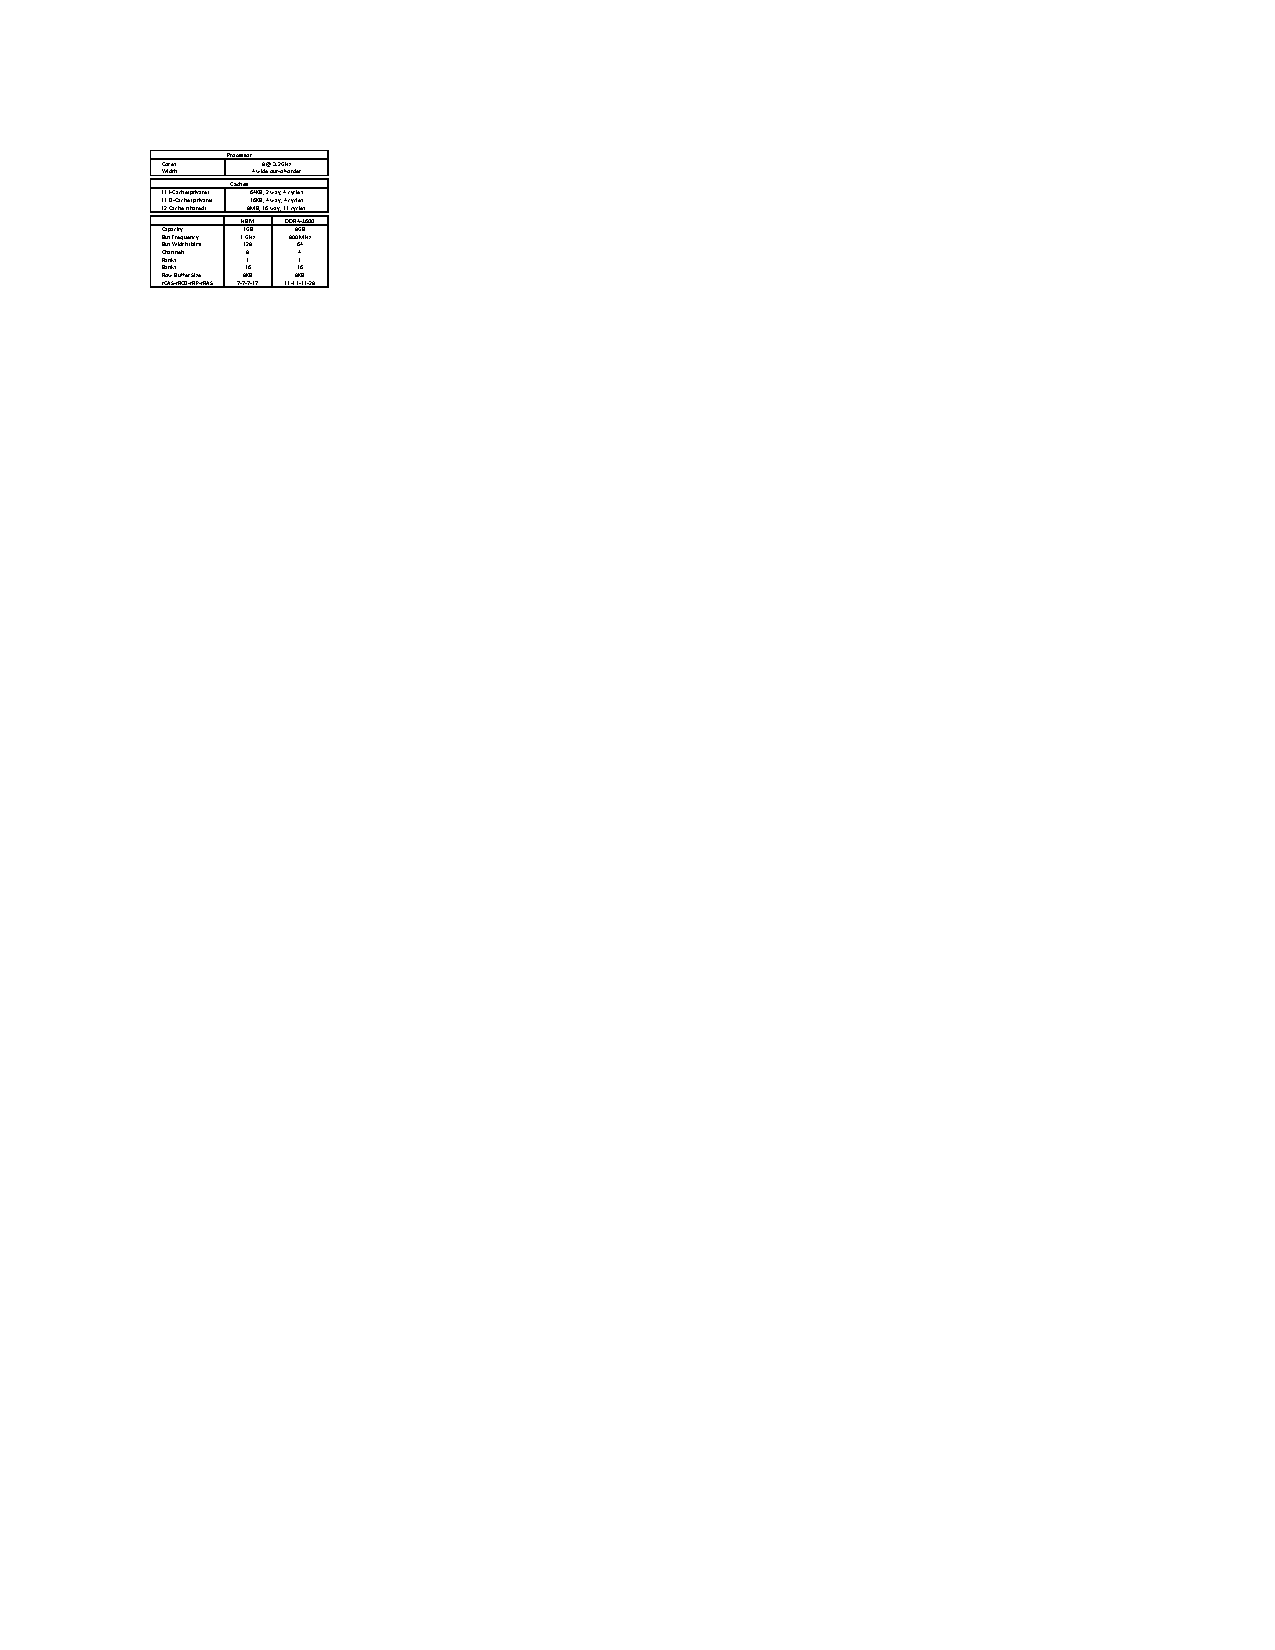
\includegraphics[width=0.46\textwidth]{figures/specs_table.pdf}
  \caption{Experimental framework configuration}
  \label{tab:specs}
\end{table}

\subsection{Experimental Methodology}
\label{sub:Experimental}

We use benchmarks from the SPEC2006 suite \cite{spec} as our workloads. Using Sniper \cite{sniper}, we recorded memory request traces while simultaneously executing 8 benchmarks on a simulated 8-core CPU. We then feed these multi-programmed memory traces into Ramulator, executing all workloads to completion. Our complete set of workloads consists of 15 ``homogeneous'' workloads, where 8 copies of the same benchmark are run in parallel (we simply refer to these workloads by the benchmark's name in later results), as well as 12 workloads featuring a random mix of 8 benchmarks each (referred to as mix1-12). Each benchmark was executed and traced under its reference input. When running homogeneous workloads, Sniper ensures that memory pages are not shared between workloads. A breakdown of the mixed workloads is shown in Table \ref{tab:workloads}.

\remark {A.P.: I'm trying to point out that same benchmarks send memory requests to different pages.}

\remark{I guarantee reviewers are going to ask -- when running 8 copies, 
did you use 8 unique inputs?}

We also extended Ramulator with cacheing for the activity tracking and/or remap tables depending on the simulated mechanism. Cache misses inject memory requests into the stream of requests fed by our trace files to retrieve the missing information. No priority is given to these cache miss requests over regular requests. When caches for hybrid memory management techniques are disabled, the simulator assumes that any information needed by any mechanism exists on chip and is accessible without any delay. The migration process was implemented in detail as well. In order to read an entire 2KB DRAM page from memory, 32 read requests need to be sent for each of the two migration candidates and then another set of 32 requests for each of the two write-backs.

As we use Ramulator with recorded traces, we chose to report Average Main Memory Access Time (AMMAT) in our results. Even though Ramulator has the ability to approximate IPC with a simple CPU model, 
AMMAT is computed with much greater fidelity with this tool,
as it models the memory system in great detail. AMMAT is the average time 
spent accessing and waiting for main memory by each request (lower is better). Due to space limitations we are not able to show results for individual workloads in most of the graphs in this paper. In those graphs, we only present the average of all mixed workloads, average of all homogeneous workloads, and overall average.

In our AMMAT experiments, we typically introduce additional accesses to the
system (migrations, bookkeeping cache misses).  The overhead of the additional
misses is accounted to the total memory stall time, but the total memory 
stall time is divided by the number of original LLC misses (main memory requests) captured in our traces
-- that is, the denominator in our AMMAT equation does not change between
experiments and equals the number of requests in our trace file.

\begin{table}
  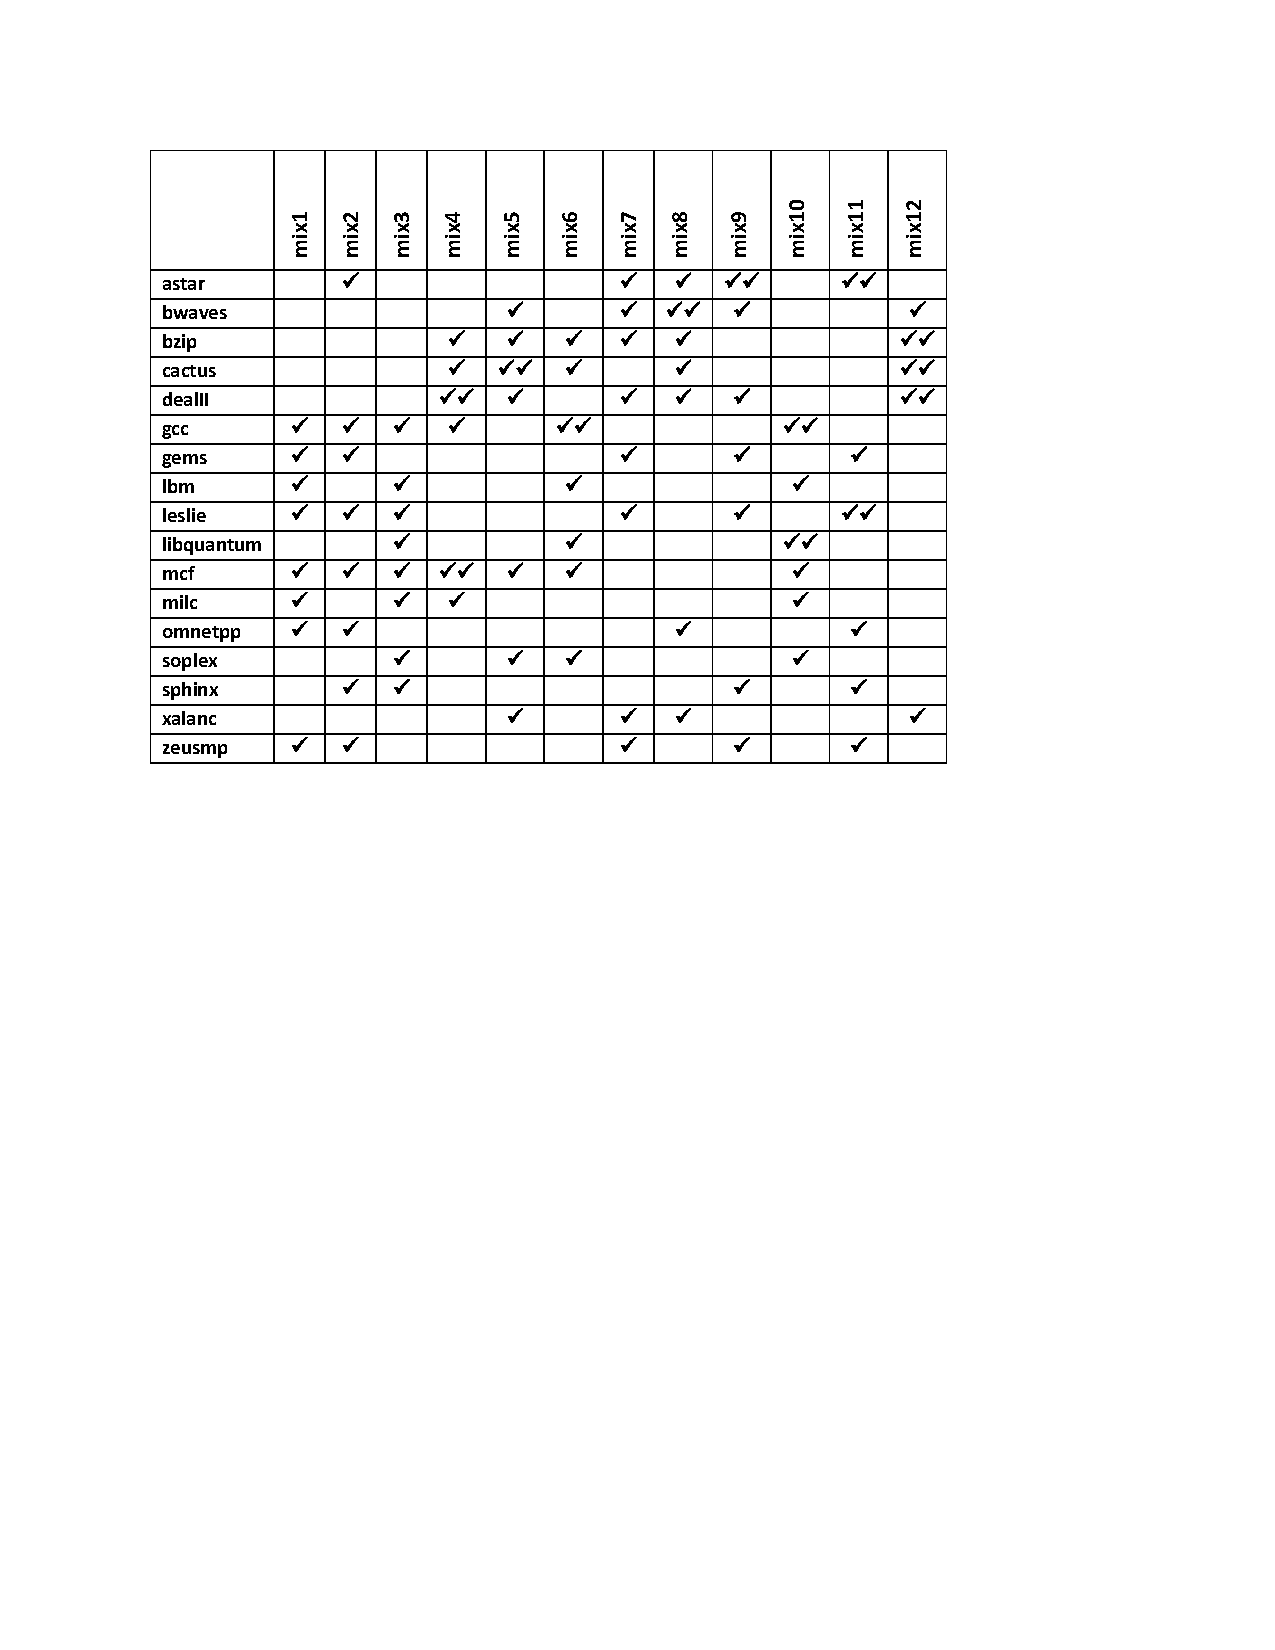
\includegraphics[width=0.46\textwidth]{figures/workloads_checkmarks.pdf}
  \caption{Mixed workloads description}
  \label{tab:workloads}
\end{table}

\subsection{Simulation Results}
\label{sub:SimResults}

\subsubsection{Page Tracking and Migration Design Space}

MemPod's activity tracking overhead and migration traffic is impacted by
the number and size of the MEA counters, as well as the epoch (interval) 
size over
which the counters accumulate.  We examine each of these design space
parameters in this section.
The number of MEA counters dictates the highest possible number of 
migrations that can be performed at each interval by each Pod, while the epoch length will determine MemPod's ability to better adapt to phase changes in a workload. The size of each MEA counter sacrifices accuracy when smaller counters are used 
but can also save space on the chip.  For these initial experiments,
the epoch length was 200$\mu$s. 

We first examine the number of MEA counters, by keeping the epoch length constant and exponentially increasing the number of counters from 16 to 512. In order to minimize the impact of other factors, we execute this experiment with 16 bits per counter and remap table caches disabled. 
%In other words, each counter was given more than enough space and all required information such as the remap table resides entirely on the chip and is accessible at no cost. 

Figure \ref{fig:num_counters} shows AMMAT normalized to the case when 16 counters are used, along with the average number of migrations per Pod per epoch (secondary axis). The results indicate that each Pod does utilize the higher number of counters and consequently perform more migrations per interval. However performance is degraded due to the overhead of migrations when more than 128 counters are used. Using 128 counters, AMMAT is improved by 6\% over the baseline with 16 MEA counters. 

\begin{figure}[h]
	\centering
  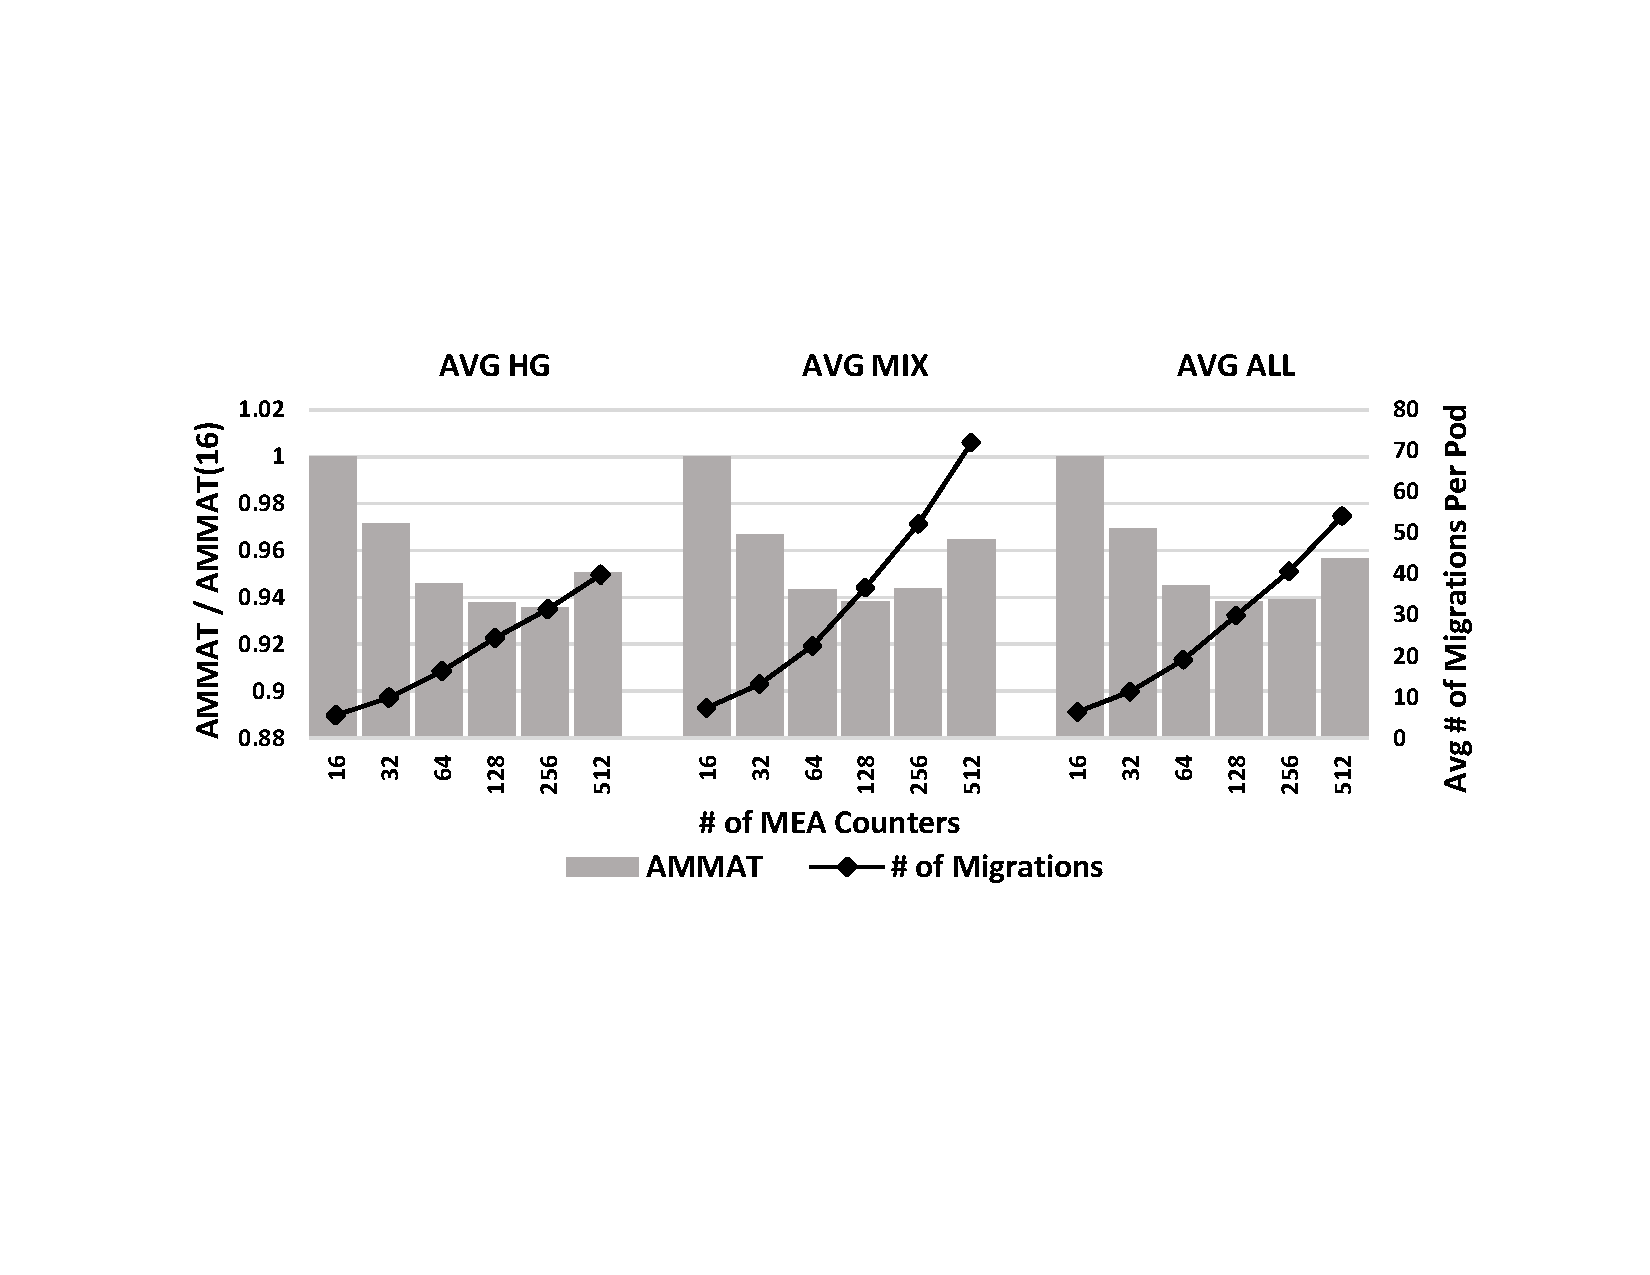
\includegraphics[width=0.46\textwidth]{figures/revised/old/num_mea.pdf}
  \caption{\# of MEA Counters Vs Normalized AMMAT (primary axis) and average \# of Migrations per Pod per interval (secondary axis)}
  \label{fig:num_counters}
\end{figure}

Figure \ref{fig:interval} shows the same experiment, but with a varying epoch length. Remap table caches were again disabled, each counter was given 16 bits and the number of MEA counters was set to 128. We observe that on average, MemPod reports the lowest AMMAT with interval length of 100$\mu$s (1.2\% improvement over 50 $\mu$s on average). As the interval length increases, more migrations are performed and AMMAT increases. Dropping below 100$\mu$s has a negative effect on AMMAT due to some epochs being entirely consumed by migrations. For comparison purposes, HMA \cite{meswani-HPCA21} identified the best epoch length to be 100ms (1000x larger) in order to support all the lengthy processes that take place during a migration event for that method.

\begin{figure}[h]
  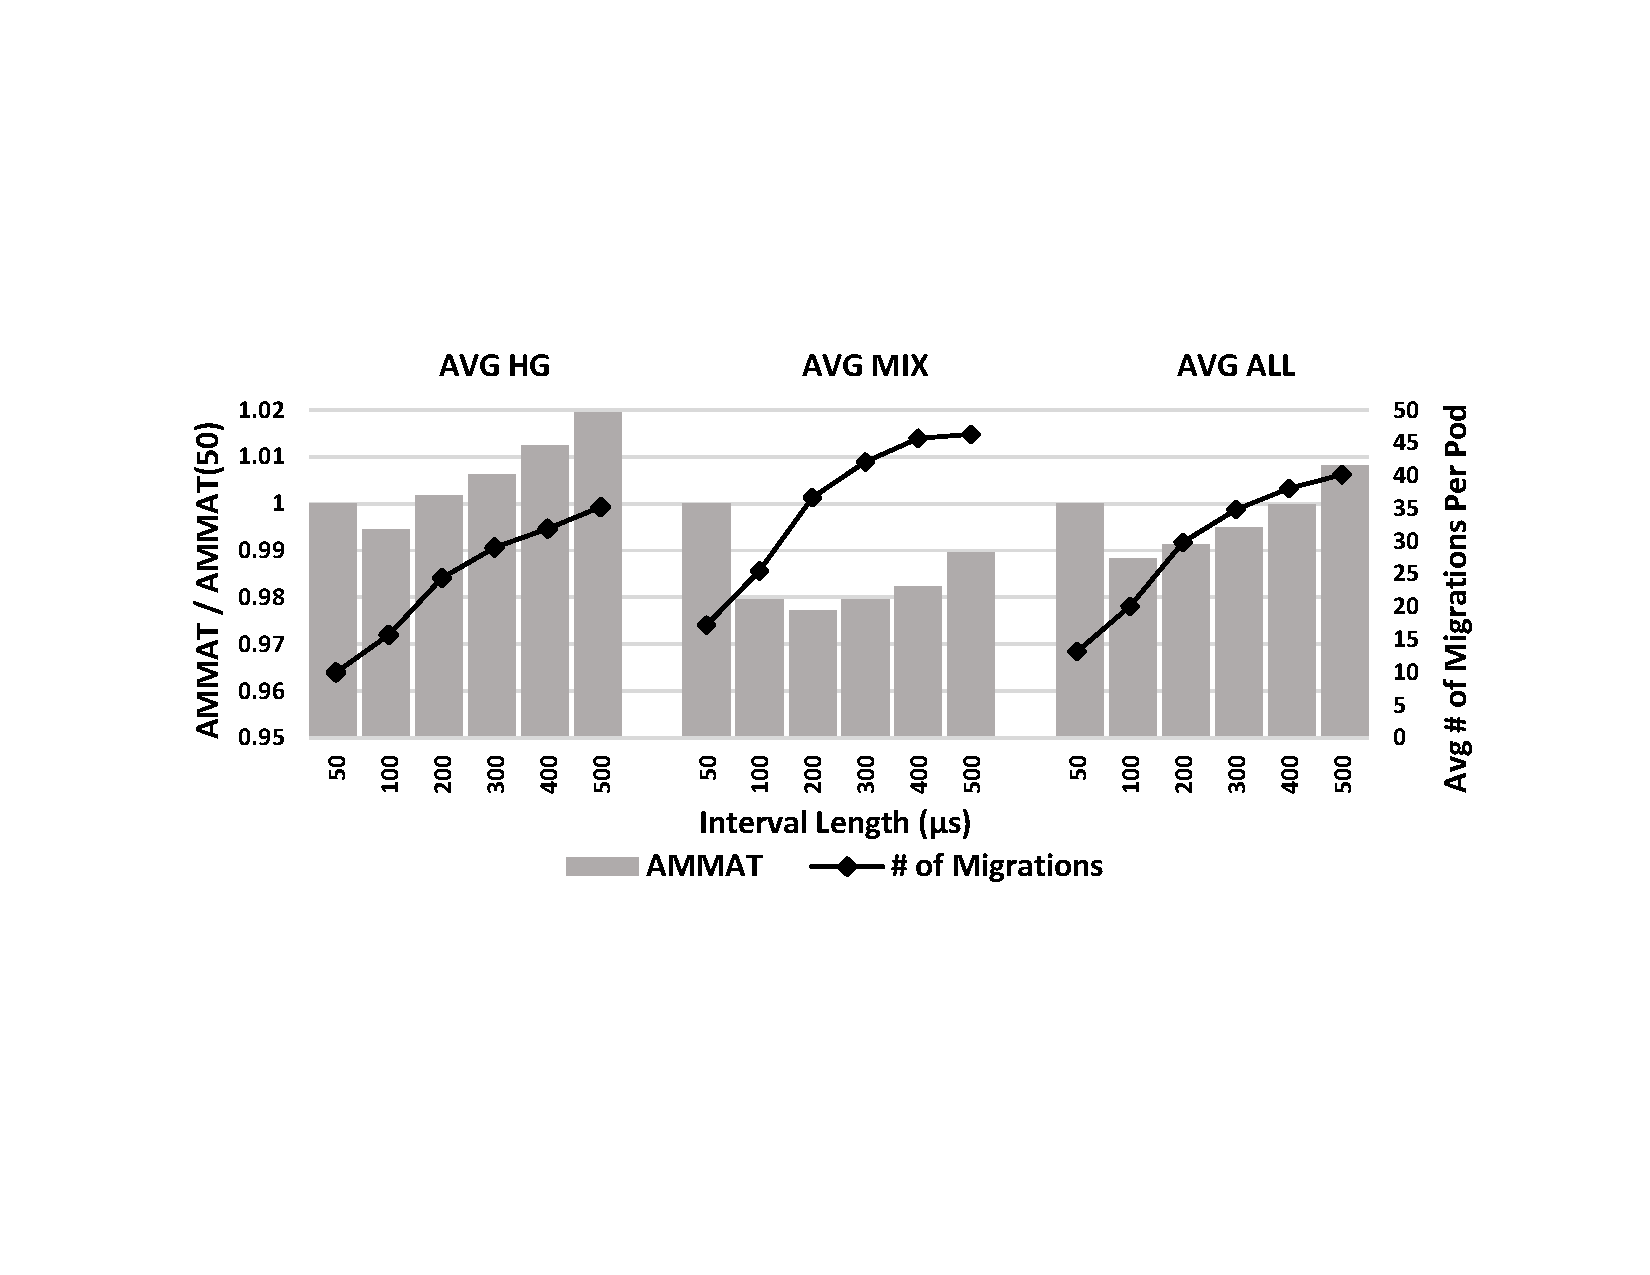
\includegraphics[width=0.46\textwidth]{figures/revised/old/interval.pdf}
  \caption{Interval Length Vs Normalized AMMAT (primary axis) and average \# of Migrations per Pod per interval (secondary axis)}
  \label{fig:interval}
\end{figure}

The size (in bits) of each counter defines the area requirements of our MEA tracking mechanism. \remark{Nuwan's comment on next sentence:\\I don't understand what this sentence is trying to say. Please reword/clarify. Why do we not saturate the counters instead of overflowing?\\A.P.: Not sure I understand this comment.} 
\remark{Dean -- my same question -- why don't we use saturating counters???}
%We modified MEA to remove map entries with counter values equal to or less than zero (instead of strictly equal to zero) in order to support counter saturation. We opted not to immediately remove an overflowed counter even though its value is now zero, as the existence of the correct counter set is crucial to the algorithm's accuracy. For this experiment we used the optimal parameter values identified in the previous experiments and set the number of MEA counters to 128 and interval length to 100us. 
%All caching was disabled in order to study the direct impact of this variable.

Figure \ref{fig:counter_size} presents the impact of counter size on AMMAT and average number of migrations. We see only minor differences in these results,
in large part because of the competing effects of accurate counting (with
large counters) and more temporal effects (with small counters).
The small counters better capture recency, because with small counters it
requires fewer divisions \remark{A.P.: Is ``divisions'' the correct word here?} to eliminate a high-access page from the pool and
replace it with a new page.  We do see a definite sweet spot at 4 bits,
where both effects seem to be in play.  We confirmed this by re-running the
experiments in Section~\ref{sec:MEA} with 4-bit instead of 16-bit counters,
and saw that prediction accuracy did improve slightly.  Although the marginal
gains are small, we use 4-bit counters in our subsequent experiments.


We first observe that 8 bits are sufficient for our workloads, as larger sizes report identical results. Our second observation is that two bit counters report a negligible performance degradation (0.3\% on average) \remark {A.P.: It's not a degradation over 8 bit counters but an improvement. Changed the sentence to compare with 4 bit counters but we might want to discuss the AMMAT improvement compared to 8 bit} over 4 bit counters and a reduced average number of migrations.

\begin{figure}[h]
  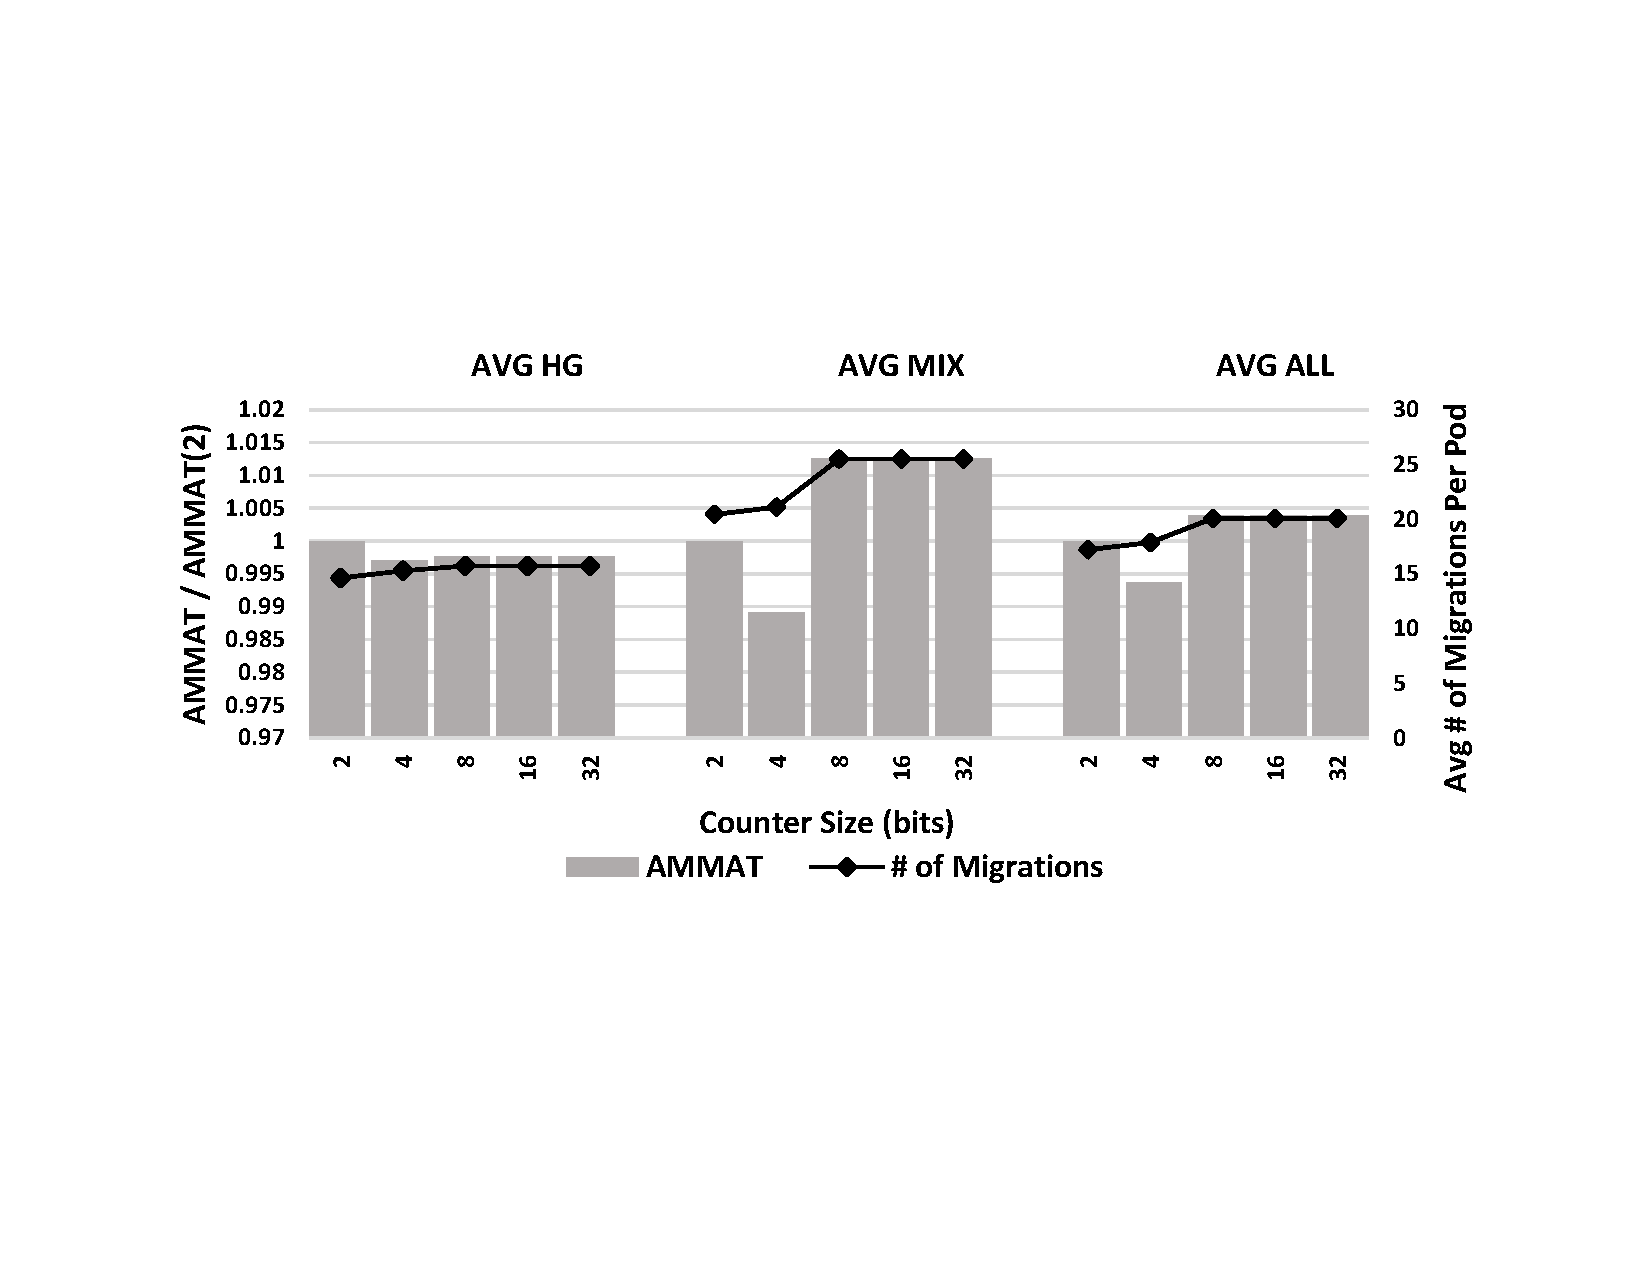
\includegraphics[width=0.46\textwidth]{figures/revised/old/ctr_size.pdf}
  \caption{Counter size (in bits) Vs Normalized AMMAT (primary axis) and average \# of Migrations per Pod per interval (secondary axis)}
  \label{fig:counter_size}
\end{figure}

The most interesting observation comes from assigning 4 bits to each counter. On average, performance is boosted slightly (up to 3\% and 0.6\% on average) even compared to using larger counters, while migration count is low. %Since a difference is observed, we can conclude that these smaller counters ``lose'' information that in turn benefits overall execution. The reported result is a welcomed artifact of the MEA algorithm combined with application behavior. 

Based on our results, we identify 4 bits per counter to be the optimal value. Each one of the 128 MEA entries needs 21 bits for addressing the 1.1M pages per Pod and 4 bits for its counter, leading to an area cost of only 400B (128 MEA counters $\times$ 25 bits) per Pod and $\sim$1.5KB total. Compared to the state of the art, MemPod's activity tracking requirement is $\sim$341x smaller than THM's (512KB) and $\sim$6000x smaller than HMA's (9MB).

\subsubsection{Performance Comparison}
\label{sub:performance}

\begin{figure*}[t]
  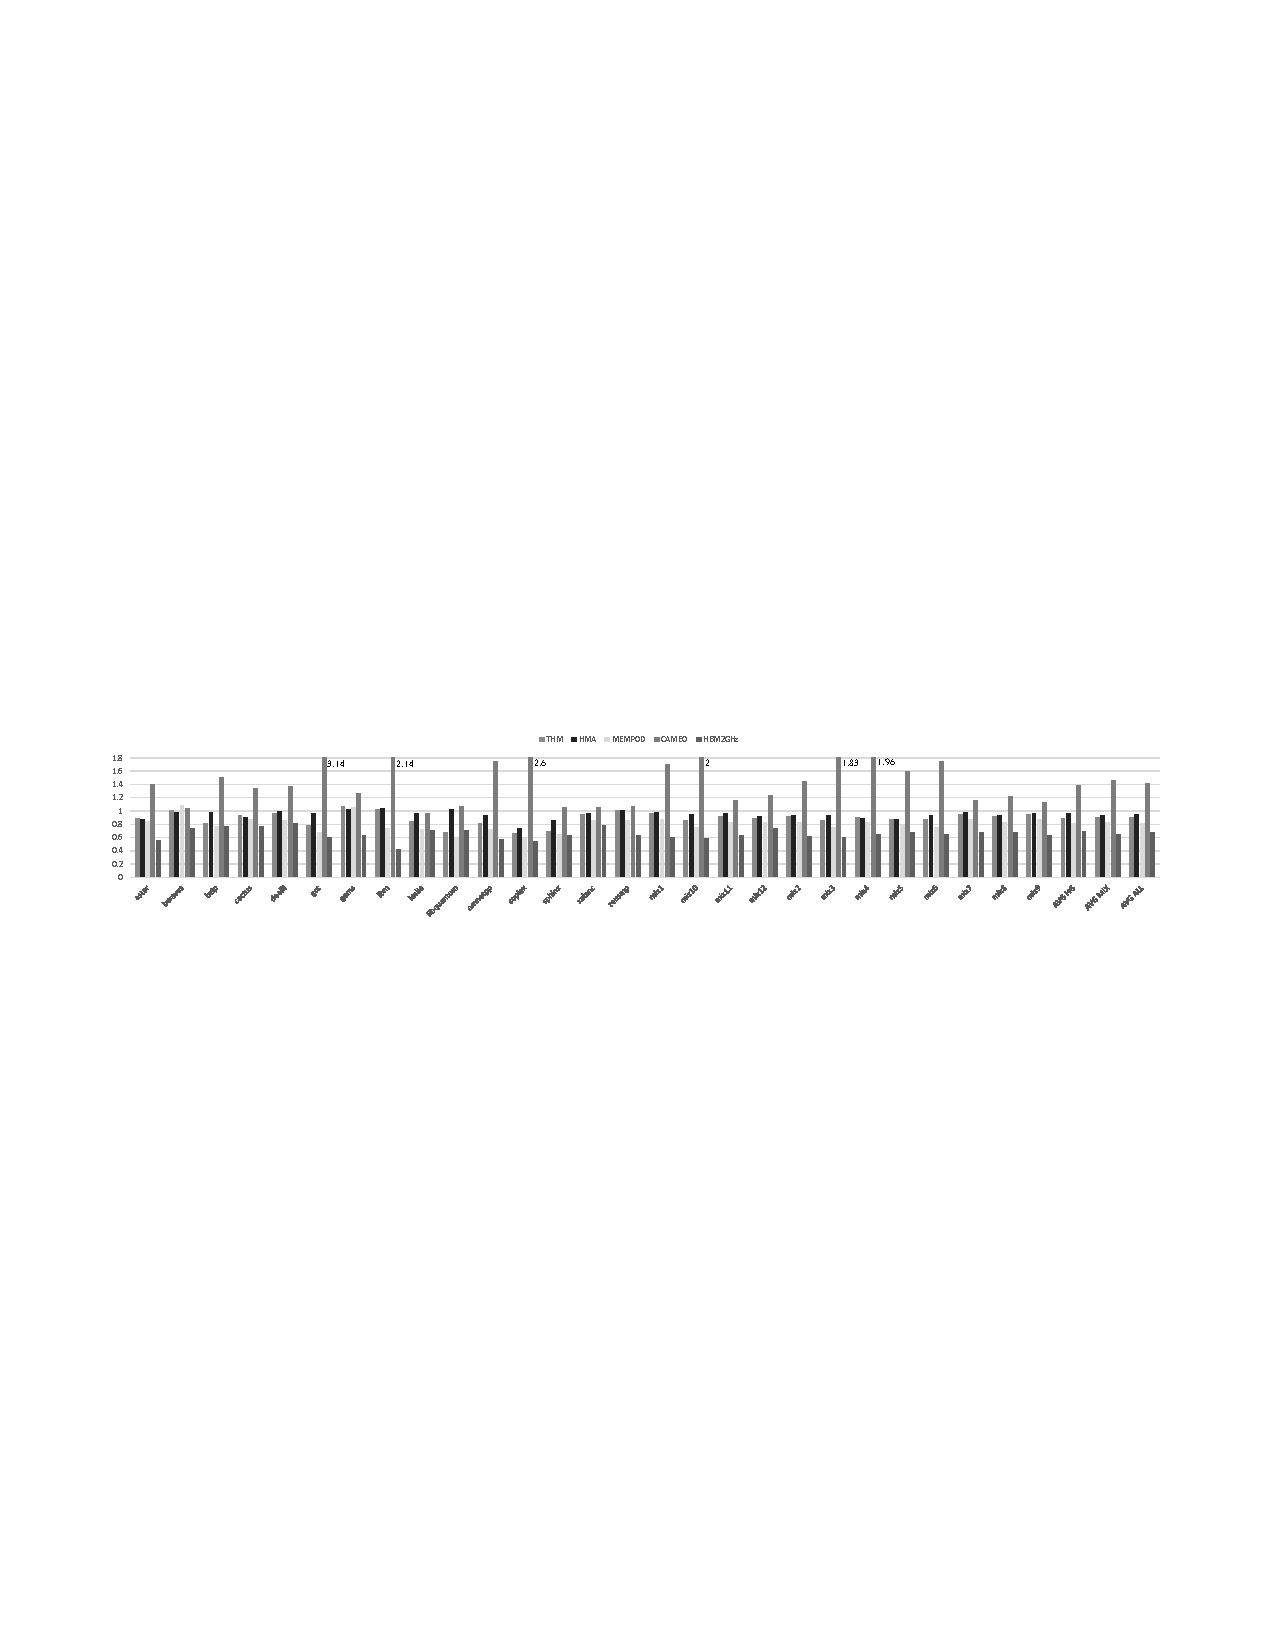
\includegraphics[width=\textwidth]{figures/revised/old/comparison_no_cache.pdf}
  \caption{Performance Comparison: AMMAT is normalized to a hybrid memory without any migration mechanism.}
  \label{fig:performance}
\end{figure*}

Figure \ref{fig:performance} presents a performance comparison of MemPod, HMA, THM, CAMEO and a configuration with 9GBs of on-chip HBM memory, normalized to the performance of a hybrid memory configuration without migration capabilities. We evaluated all mechanisms with caching disabled. 

Based on the results we derive some interesting observations:
\begin{itemize}[leftmargin=0.4cm]
\setlength\itemsep{0em}
	\item MemPod outperforms the state-of-the-art competitors in the majority of our workloads, and in several cases scoring very close to an HBM-only configuration. 
	\item On average, CAMEO reports AMMAT degradation by 41\% over the no-migration scheme. The negative impact is caused by our high slow:fast memory capacity ratio leading to intra-segment conflicts. Larger segments also counteract the application's spatial locality benefits, causing a ping-pong effect. From our experiments, we observe CAMEO to be the leading mechanism regarding the amount of data moved between memories, moving 3.9GB of data on average per 8-core experiment. For comparison purposes, MemPod moved 3GB on average, however migration traffic was divided between Pods, resulting in 790MB per Pod. THM moved 865MB on average and finally HMA moved 578MB due to its large intervals. We also frequently observed redundant migrations with CAMEO, where a line is evicted shortly after migration without being touched in the time it spent residing in fast memory. Optimizations such as intellingent line allocation to segments can significantly improve CAMEO's performance and reduce intra-segment conflicts, however to maintain a fair evaluation, CAMEO is evaluated under the same memory organization as the rest of the mechanisms.\remark {A.P.: Should we make this a subsection on its own?}
	\item On average MemPod reports 21\% higher AMMAT than HBM-only, while THM and HMA report 33\% and 40\% respectively.
	
	\item In some workloads migration overall is harmful to performance, 
as observed with the gems and bwaves workload, where a no-migration scheme reports 
higher performance (lower AMMAT). We observe that in those cases, MemPod leads to deteriorated performance compared to the other mechanisms. However, in the cases of lbm and zeusmp, 
MemPod increases performance, while THM, HMA and CAMEO report higher AMMAT than the no-migration scheme.

	\item HMA and MemPod outperform HBM-only when executing the libquantum experiment. In the case of libquantum, the working set size fits entirely in our fast memory. As a result, after some migrations, the entire working set will be present in HBM.  With an HBM-only system and no migrations, pages
are inserted sequentially by address.  In a migration-based system, 
simultaneously-hot pages are inserted together after each epoch.  As the
DRAM row buffer is bigger than a page, we find that the co-location of
simultaneously-hot pages increases row buffer hit rate from 7\% (HBM only)
to 90\% (MemPod), with 87\% of those taking place in fast memory.  HMA also sees an improvement in row buffer hit rate. THM and CAMEO cannot take advantage of the small footprint due to their restricted migration flexibility (only one hot page/line per segment can reside in fast memory).
\remark{Don't know how to explain THM, but the effect is smaller -- what is
the row buffer hit rate?\\A.P.: THM's results were wrong. The updated results and graph show that it doesn't outperform HBM.}
%However, correct timing is the driving factor behind this impressive performance increase. Our results show the row-buffer hit ratio to be \TODO{??x} times higher than the HBM-only memory system (and random page assignment). Apparently, page migrations resulted in an in-HBM page order that increases page hits and exploits a much higher degree of memory parallelism from the application. This result could be further explored and intentionally recreated in some future work.
\end{itemize}

\subsubsection{Caching Effect}
\ignore{
\begin{figure}
  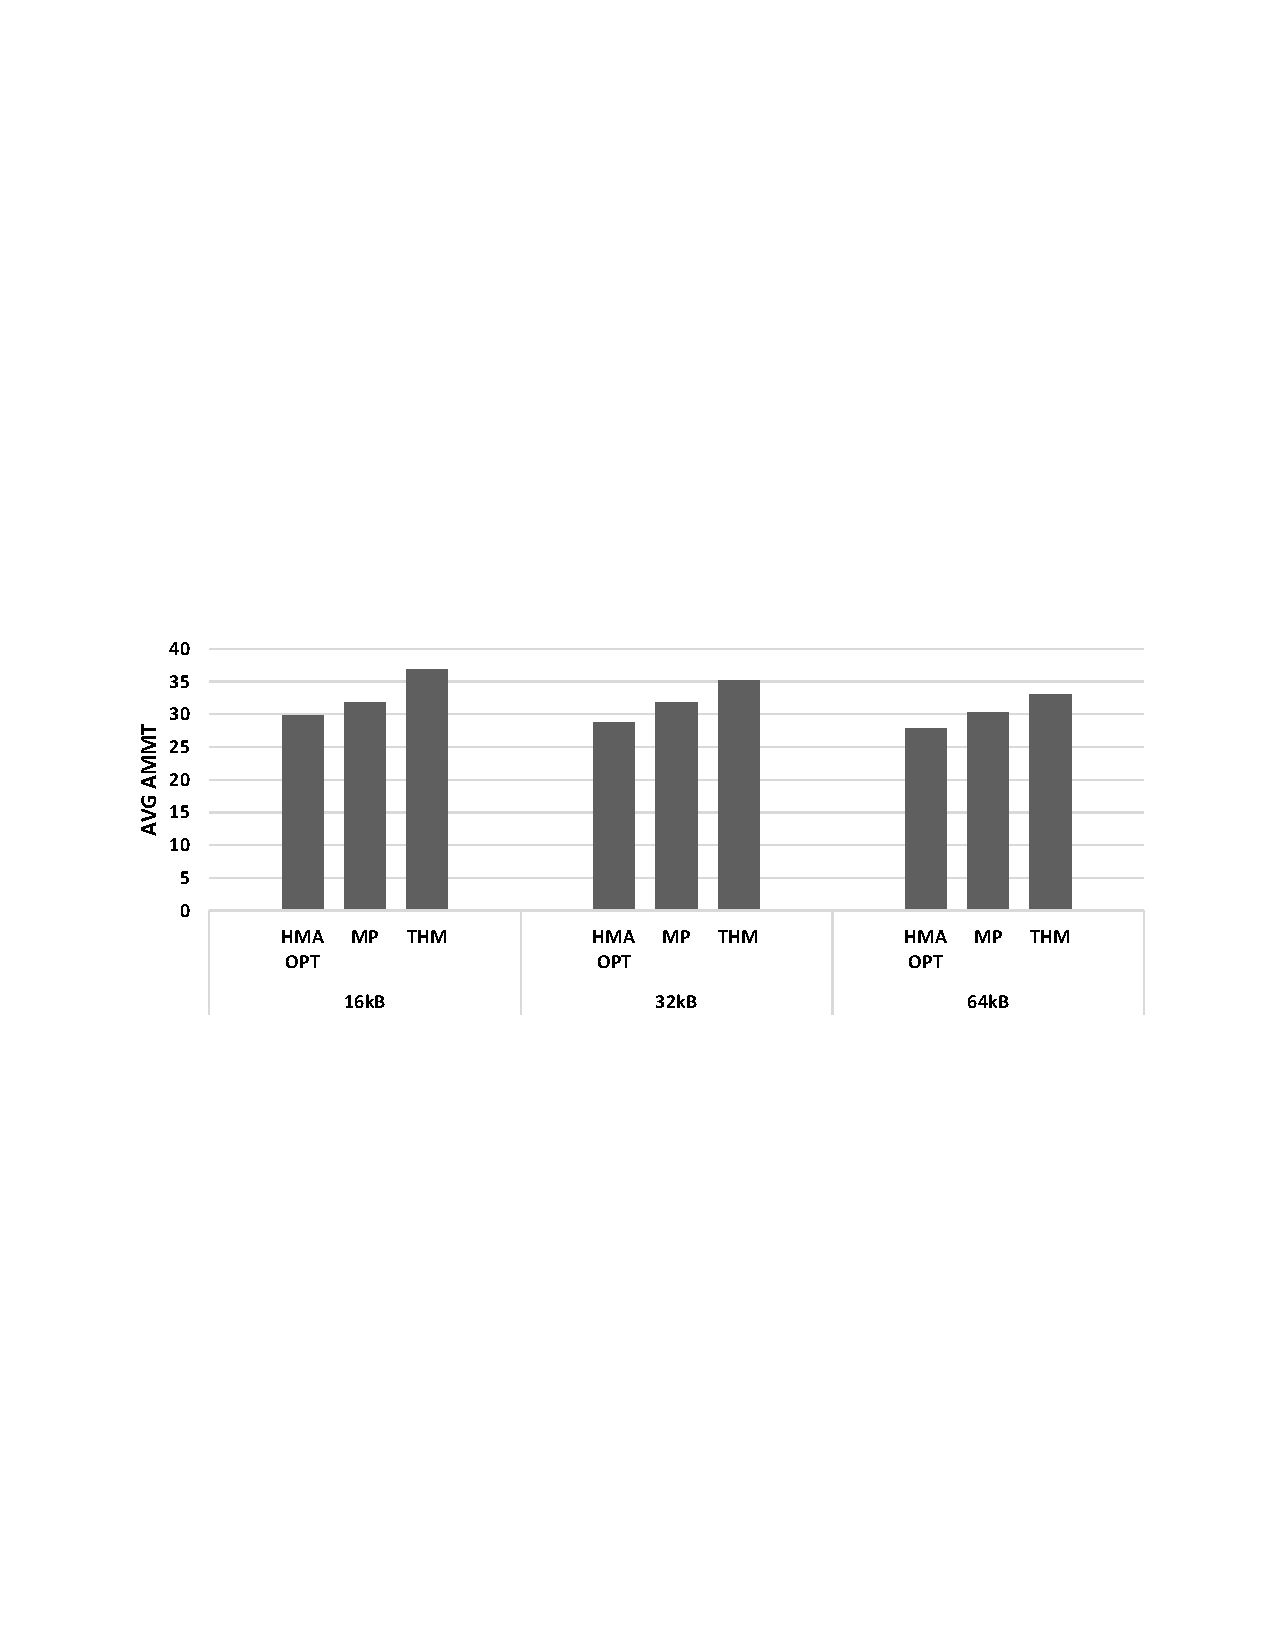
\includegraphics[width=0.46\textwidth]{figures/cache_impact.pdf}
  \caption{Cache Impact. AMMAT normalized to stock TLM (no migrations)}
  \label{fig:cache}
\end{figure}

\remark{A.P.: I don't have CAMEO results with caching yet. Not sure if it will be ready on time but I'm working on it.}

\remark{A.P.: Need to change the structure of this section due to issues with results.}


Migration mechanisms will be forced to include a cache as activity tracking and remap table structures are too large to store on-chip. The use of a cache will unavoidably hinder performance. In this experiment we evaluate the impact of a cache on each mechanism's performance. As described in Section \ref{sec:Architecture}, each mechanism has different cache requirements. THM caches its counters and remap table together with its SRT structure. HMA has no need for a remap table but has high storage requirements for its counting mechanism. MemPod must cache only its remap table as MEA counters will be on chip. We simulated each mechanism with 16, 32 and 64 KB of cache. For MemPod, the available cache capacity was divided equally over four Pods. All mechanisms use the stacked memory as backing store for their tracking information.

HMA's design further complicates this study, as sorting all activity counters at each epoch is performed by the OS, utilizing the cpu's cache instead of the dedicated migration cache. In our results, we present ``HMA-OPT'', an HMA flavor that does not take into account any penalties for OS interrupts, TLB shootdowns, Page Table (PT) updates, walks and misses, or sorting of the large
pool of counters.
We also do not model the application-level effects of starting with a cold TLB after each interval.

Figure \ref{fig:cache} shows our results obtained by taking the average AMMAT from all our workloads for each mechanism. HMA-OPT reports the lowest AMMAT, albeit unrealistic and MemPod outperforms every other mechanism regardless of the cache size. MemPod outperforms THM by 9\% with a 64kB cache, while HMA-OPT outperforms MemPod by 9\%.
}

Migration mechanisms will be forced to include a cache as activity tracking and remap table structures are too large to store on-chip. The use of a cache will unavoidably hinder performance. As described in Section \ref{sec:Architecture}, each mechanism has different cache requirements. THM caches its counters and remap table together with its SRT structure. HMA has no need for a remap table but has high storage requirements for its counting mechanism. MemPod must cache only its remap table as MEA counters will be on chip. 

In this experiment we evaluate the impact of a cache on MemPod's performance. We simulated the optimal MemPod configuration identified over the course of this section with 16, 32 and 64 KB of cache. The available cache capacity was divided equally over four Pods. We implemented MemPod's caching logic to use the stacked memory as backing store, leading to 2.8MBs per Pod to be dedicated for this purpose for an overall 1\% reduction of the available stacked memory capacity.

In our implementation, each cache miss injects a read request to retrieve missing data. Since all of MemPod's cache misses will occur due to Remap Table updates or lookups it becomes a blocking request for the affected Pod. All incoming traffic needs to be delayed until the missing data is retrieved. In-flight requests are not affected by incoming cache misses. Each Pod operates (and blocks) independently allowing other Pods to continue servicing incoming traffic.

\begin{figure}
  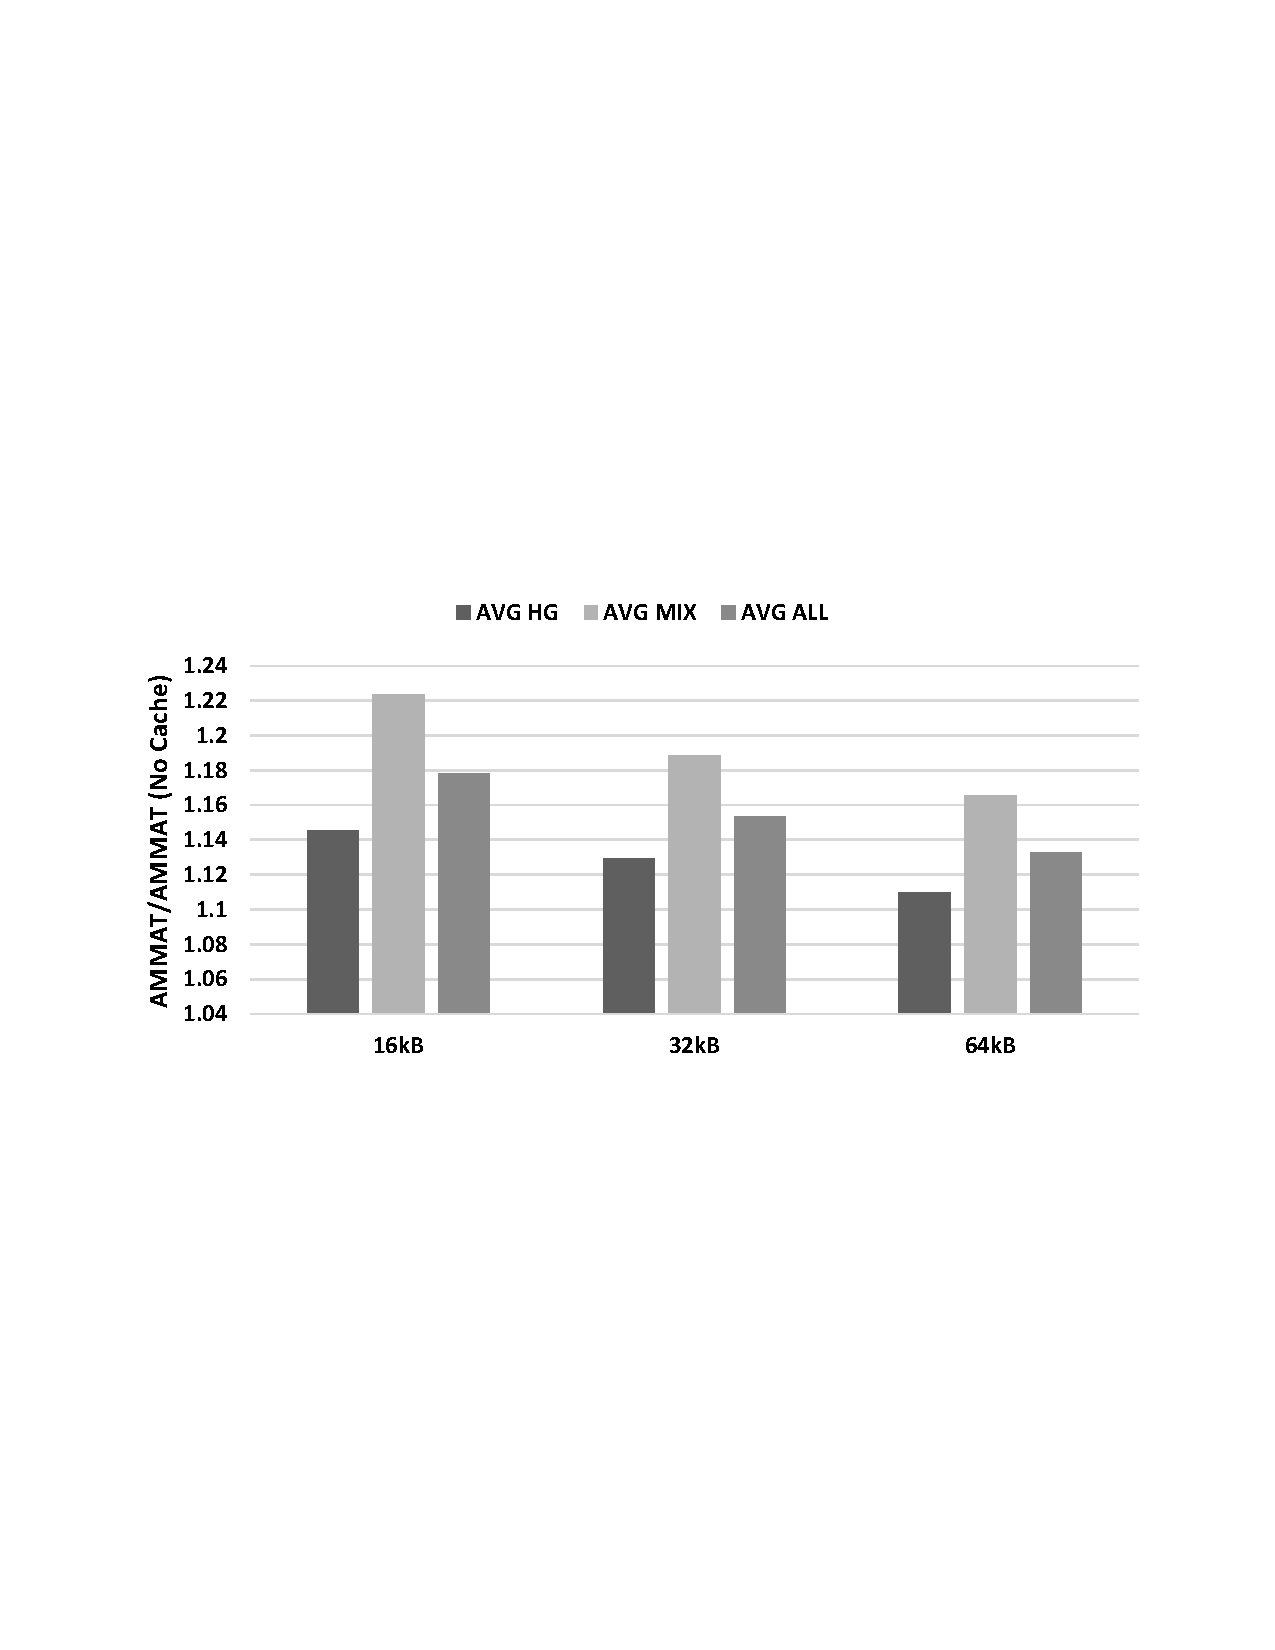
\includegraphics[width=0.46\textwidth]{figures/revised/old/cache_impact.pdf}
  \caption{Cache Impact. AMMAT normalized to stock MemPod (no cache)}
  \label{fig:cache_impact}
\end{figure}

\begin{figure}
  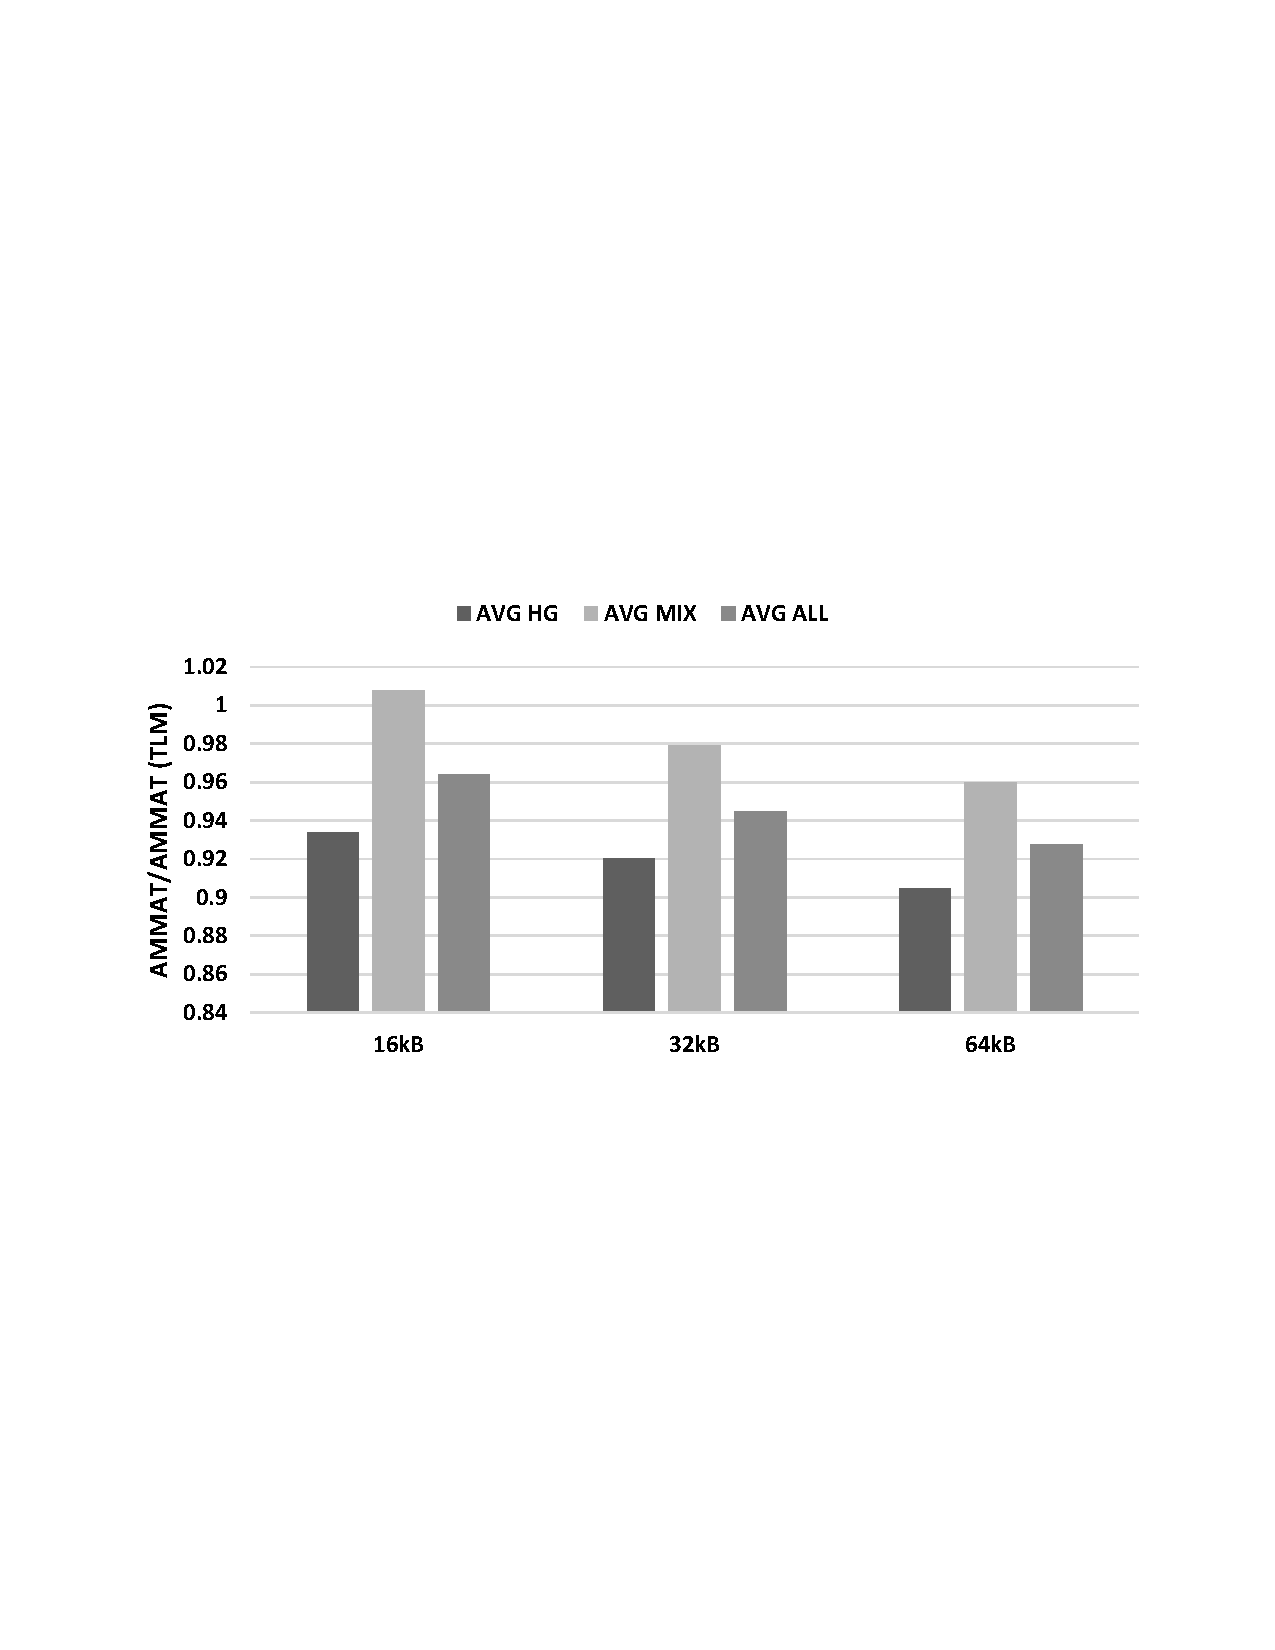
\includegraphics[width=0.46\textwidth]{figures/revised/old/cache_norm_tlm.pdf}
  \caption{Cache Impact. AMMAT normalized to stock TLM (no migrations)}
  \label{fig:cache_norm_tlm}
\end{figure}

Figures \ref{fig:cache_impact} and \ref{fig:cache_norm_tlm} show our results obtained by taking the average AMMAT from all our workloads for each cache size. Figure \ref{fig:cache_impact} shows the obtained average AMMAT normalized to MemPod's performance without a cache. For 16, 32 and 64kB of cache, the impact on MemPod's performance is 18, 15 and 13\% respectively. Figure \ref{fig:cache_norm_tlm} shows our results normalized to a two-level memory configuration without any migration mechanism. With 16, 32 and 64kB of cache, MemPod reports 3.6, 5.6 and 7.3\% AMMAT improvement.

The cache impact is significantly high mainly due to the blocking nature of cache misses. However, a less conservative design could reduce this effect by allowing incoming requests to proceed if they do not depend on any missing information, at some hardware cost. Better cache organization could also help alleviate the issue.

\subsubsection{Scalability}

\begin{figure}
  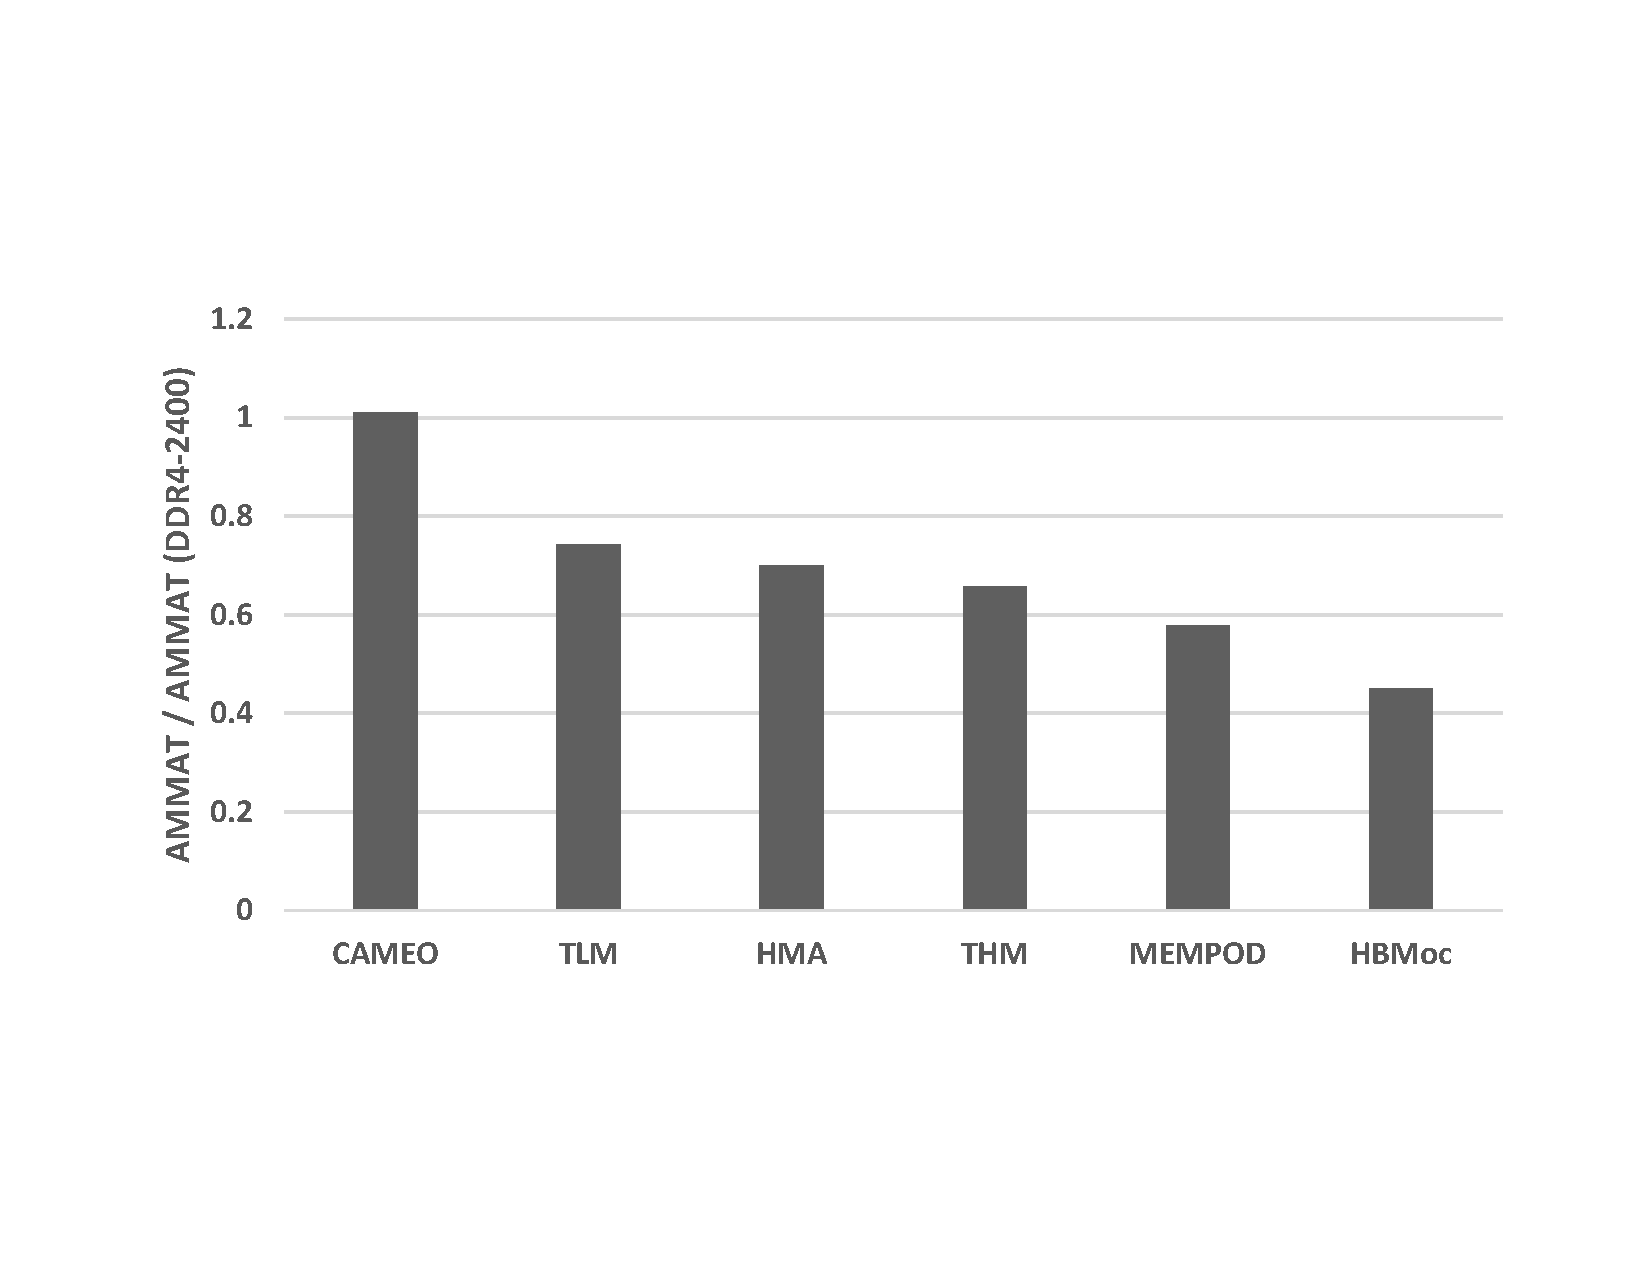
\includegraphics[width=0.46\textwidth]{figures/revised/old/scalability_speed.pdf}
  \caption{Scalability to faster memories. AMMAT normalized to a DDR4-only memory.}
  \label{fig:scalability}
\end{figure}

MemPod is designed to be scalable with future technology.  If we grow memory
sizes by increasing the number of pods, the size of the remap table and the 
size of the MEA counters will remain constant (per pod, and thus per memory
page) if the memory per pod remains constant.  If instead we increase
memory capacity per pod, the size of the remap table (per memory page)
will go up only with the log of the per-pod memory. If we choose to scale
the number of counters with the size of memory per pod, it will go up
similarly; however, if we do not scale up the counters at the same rate
(e.g., four times the memory, but double the counters), then the cost
of the counters (per memory page) will go down.

Additionally, the memory traffic caused by migrations will remain distributed
and off the primary processor interconnect.

We also expect the latency differential between main memory levels to 
continue to grow.  This will happen as 3D memory parts mature, and as
we integrate new memory technologies into the system (e.g. hybrid
volatile and non-volatile memory systems).
To examine this, we model a system where both the 3D DRAM and the DDR memory
are faster, but the 3D DRAM is accelerated further resulting in a higher
latency ratio between the two. 
In particular, we simulate a 4GHz HBM as our stacked memory and a DDR4-2400 as our off-chip memory. 
We assume no cacheing effects in this experiment.
Figure \ref{fig:scalability} shows our AMMAT results, normalized to a configuration with 9GBs of off-chip DDR4-2400. The label ``HBMoc'' shows a 9GB configuration with overclocked HBM only. We first observe that CAMEO now reports a 1\% AMMAT degradation. The increase in speed differential between stacked and off-chip memory appears to be beneficial, however we can still observe the impacts of intra-segment conflicts. Compared to a configuration with no migration support (TLM), HMA improves AMMAT by 6\%, THM by 12\% and MemPod by 22\%. The overclocked HBM-only configuration is 40\% faster compared to TLM.

\ignore{
We first observe that HMA-OPT due to its high number of 
migrations and low prediction accuracy increases AMMAT by 8\% compared to a 
Two-Level Memory without migration (TLM). THM and MemPod reduce AMMAT by 13\% and 24\% respectively, compared to TLM. With this memory configuration, MemPod 
reports AMMAT improvements of 42\% over HMA-OPT, and 15\% over THM. 
}

